\documentclass[a4paper]{report}
\usepackage[a4paper,bindingoffset=0.2in,%
left=1in,right=1in,top=1in,bottom=1in,%
footskip=.25in]{geometry}
\usepackage{blindtext}
\usepackage{graphicx}
\usepackage{plain}
\usepackage{url}
\usepackage{pdflscape}

\usepackage[utf8]{inputenc} % Required for inputting international characters
\usepackage[T1]{fontenc} % Output font encoding for international characters
\usepackage{fouriernc} % Use the New Century Schoolbook font

%\title{Full Unit Project: Building a Game}
%\author{Supervisor: Jasper Lyons}
%\author{Pavan Jando}

%\begin{document}
	
	
	%----------------------------------------------------------------------------------------
	%	TITLE PAGE
	%----------------------------------------------------------------------------------------
	
\begin{document} 

\begin{titlepage} % Suppresses headers and footers on the title page
	
	Pavan Jando Year 3
	
	\centering % Centre everything on the title page
	
	\scshape % Use small caps for all text on the title page
	
	\vspace*{\baselineskip} % White space at the top of the page
	
	%------------------------------------------------
	%	Title
	%------------------------------------------------
	
	\rule{\textwidth}{1.6pt}\vspace*{-\baselineskip}\vspace*{2pt} % Thick horizontal rule
	\rule{\textwidth}{0.4pt} % Thin horizontal rule
	
	\vspace{0.75\baselineskip} % Whitespace above the title
	
	{\LARGE CS3821\\ FULL UNIT PROJECT\\ BUILDING A GAME\\} % Title
	
	\vspace{0.75\baselineskip} % Whitespace below the title
	
	\rule{\textwidth}{0.4pt}\vspace*{-\baselineskip}\vspace{3.2pt} % Thin horizontal rule
	\rule{\textwidth}{1.6pt} % Thick horizontal rule
	
	\vspace{2\baselineskip} % Whitespace after the title block
	
	%------------------------------------------------
	%	Subtitle
	%------------------------------------------------
	
	Year 3 Final Project % Subtitle or further description
	
	\vspace*{3\baselineskip} % Whitespace under the subtitle
	
	%------------------------------------------------
	%	Editor(s)
	%------------------------------------------------
	
	By
	 			
	\vspace{0.5\baselineskip} % Whitespace before the editors
	
	{\scshape\Large Pavan Jando \\} % Editor list
	
	\vspace{0.5\baselineskip} % Whitespace below the editor list
	
	\textit{October 5, 2018} % Editor affiliation
	
	\vfill % Whitespace between editor names and publisher logo
	
	%------------------------------------------------
	%	Publisher
	%------------------------------------------------
	
	
	\vspace{0.3\baselineskip} % Whitespace under the publisher logo
	
	Supervisor \\ Jasper Lyons
	
\end{titlepage}


%\maketitle
\renewcommand{\thesection}{\arabic{section}}
\tableofcontents
\pagebreak

\section{Abstract}
\subsection{The Game}
I plan to make an android game that uses GPS location tracking where the player can encounter in-game enemies to battle and level up their character. The user can pick from a selection of characters which vary in abilities and play-styles. Battling AI enemies gains experience which levels their character and increases their statistics e.g. strength, speed. Enemies also have a chance of dropping items that the user can equip, utilise or trade with other players.
\\\\
Users should also be able to interact with each other by battling, trading or playing co-operatively. They can do this by grouping together for boss battles which generally would be in more popular areas such as Royal Holloway. These enemies should be stronger and more difficult to defeat but also more rewarding for defeating them.

\subsection{Aims}
The aim of this project is to develop and deploy a playable game whilst learning about the game \\development ecosystem. I will also explore the android life-cycle and how mobile games differ from PC games. There are a lot more factors to be concerned about such as battery life and performance when using less powerful hardware. I want this project to be representative of my willingness to learn technologies that are new to me and my efficiency in doing so. Knowing how to use platforms like Android Studio and programming in Unity are important skills when entering the games industry.  
\\\\
Furthermore, I will also learn about the different design patterns that are most commonly used in games such as Flyweight, Factory, Singleton and Game Loop which are just a few of many. Efficiency and well-designed algorithms are key to making a game run smoothly without affecting the user experience. For example, Flyweight is important for use in games where many objects need to be displayed all at once. It takes the similarities between these objects and extracts it to its own class. Therefore, less data is being processed and a load is taken of the CPU/GPU due to many objects sharing from the same set of characteristics. \cite{Flyweight}

\subsection{Proof of Concepts}
The end goal of my game is to have many players connecting to a dedicated server which then retrieves and stores data about theirs and other characters in a database. This will allow players to interact with each other via trading and battling. I will need to create a basic client-server model to show that I can transmit data between the client and server then also store this information in a database. A difficult part of this will be organising and scheduling requests the server gets from multiple clients and ensuring that data does not get lost in transmission. For this I will need to create a thread for each client connecting to the server to allow for continuous connection and disconnection of clients \cite{MultiClient}.  
\\\\
Some popular developing platforms for android games include Unity, Corona SDK, Unreal Engine 4 and Amazon's Lumberyard to name a few \cite{Engines}. For my needs, the users character model will be 3D, animated to walk or run depending on the user’s speed whilst moving. Corona SDK is limited to 2D development and does not help me fulfil my requirements. After doing some further research I concluded that Unity would be the ideal engine to use as it is very popular among android developers meaning there is more resources to learn from \cite{Unity}. Lumberyard is relatively new and has not yet been widely adopted as the likes of Unity. Unreal Engine is a good alternative but again I felt that many sources encouraged Unity especially for beginner game developers such as myself. 
\\\\
Another decision that needed to be made was which mapping software would be ideal. I narrowed my search to OpenStreetMap (OSM) and Google Maps (GM) as I felt these were the most popular mapping tools used by developers for their accuracy and large amounts of data. The main difference between the two is that OSM is open versus GM being closed source. This mainly means there is less control over data and any customisations with using GM over OSM \cite{Maps}. I discovered that OSM API is not as clear and easy to read as the GM API \cite{API}. However, I was able to find some examples to learn from which were clearer \cite{github}. Taking these factors into consideration I have decided to use OSM for its superior control of data and customisations.

\begin{landscape}
\section{Timeline}
\begin{figure}[!h]
	\centering
	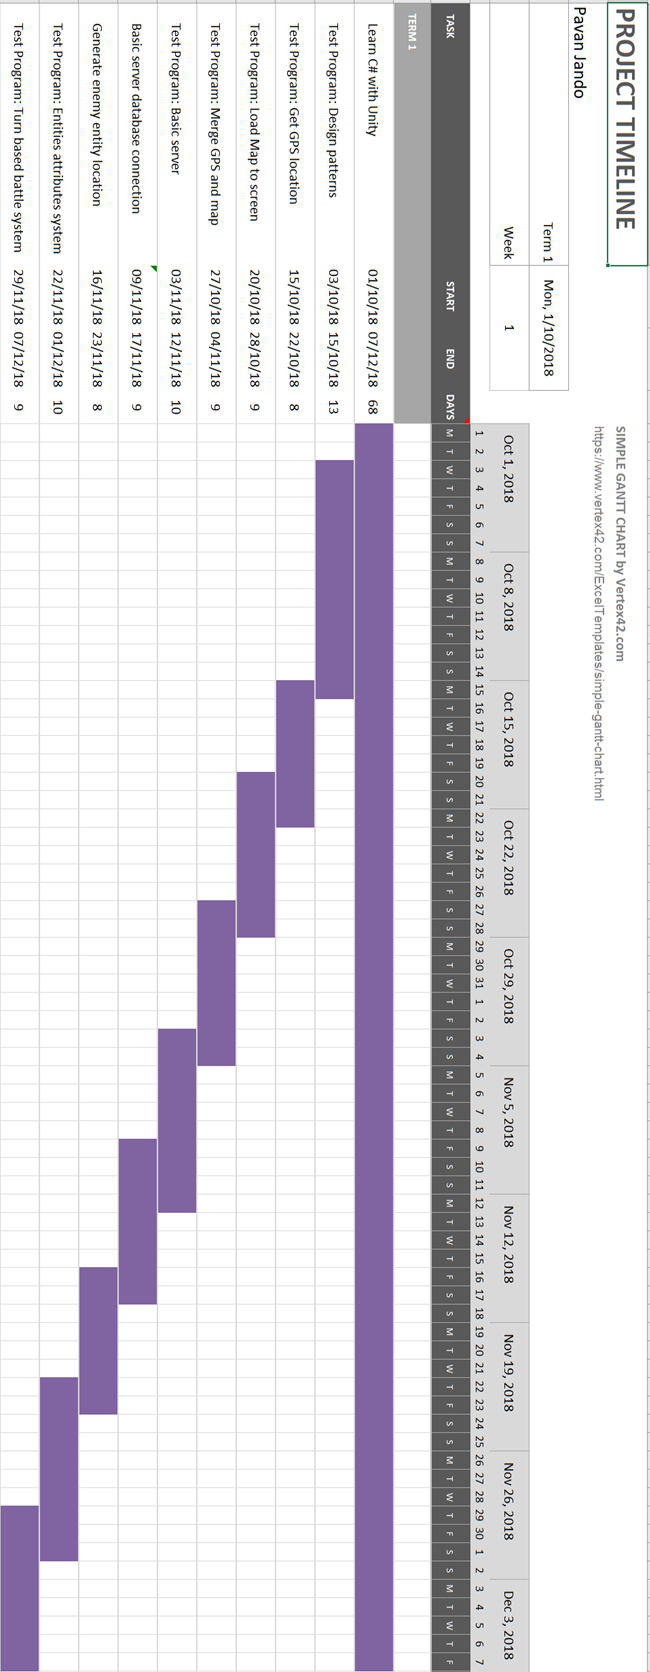
\includegraphics[scale=0.80, angle=90,]{term1}
	\caption{Term 1 Gantt Chart}
	\label{fig:term1}
\end{figure}
\pagestyle{empty}
\newpage
\pagestyle{empty}
\begin{figure}[!h]
	\centering
	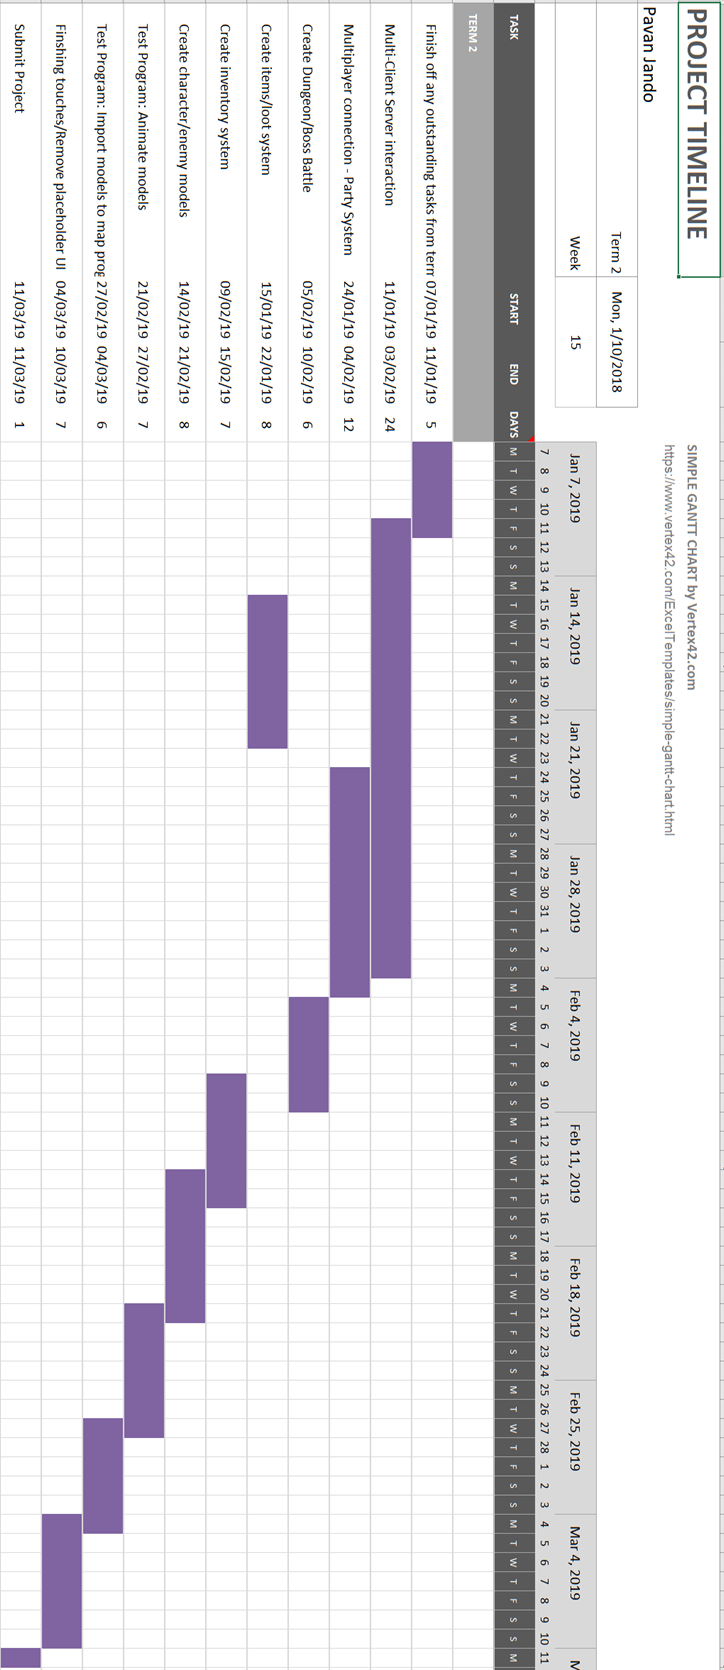
\includegraphics[scale=0.82, angle=90]{term2}
	\caption{Term 2 Gantt Chart}
	\label{fig:term2}
\end{figure}
\end{landscape}

\newpage
\subsection{Milestones}
As shown in my Gantt chart, each "Test Program" is a milestone for me as it shows that I am able to learn a new concept or use a new technology. With these milestones completed it is proof that I am able to do a lot of the work that is required to make this game. For example, being proficient in C\# using the Unity environment is a key skill to that needs to be of a high enough standard to complete the project. This is why I will be using it in the "Test Programs" that have been labelled.
\\\\
An essential milestone for me is to be able to use the fundamental game design patterns in a language I have not used before. This will be proof of my ability to confidently program using C\#. Such a pattern is the Game Loop which exists in nearly all games. One iteration of the loop represents one frame being drawn according to any user input \cite{Loop}. It updates the game state and renders it to the screen. Therefore it is crucial each iteration is fast to provide a smooth user experience.
\\\\
I have divided the work load across the two terms such that single-player will be focused on in the first term and multi-player in the second term. Multi-player is a lot of work to implement and I want to be sure that there is at least a single-player version that can be delivered by the end of the second term. 
\section{Risk Assessment}
The first risk, as in most projects, is falling behind schedule meaning key features do not get developed fully or are dysfunctional. This can happen for a plethora of reasons such as wasting time, over-ambitiousness or difficulty of the task. It is important I try to remain on task ensuring that I focus on the core features of the game and add finishing touches afterwards. I understand that my idea is ambitious and that I need to break down the game into smaller components that need to be completed before moving on to the next. For example, ensuring that the game works as a single-player game before moving towards multi-player. If I fail to keep up with my schedule, I will need to revise my plan and decide which features take priority and need completing first.
\\\\
As previously discussed, I will be using OSM over GM to get my map data from. The risk is that the API looks difficult to use as it is not as clear as the GM API. After doing more research I found a few more resources that I can learn from to help me progress forward \cite{github}. However, if I decide in future that it is necessary to change mapping software I will create an adapter class to decouple my code base and the mapping software. This way the only thing that needs changing is the adapter class and it should not affect the entire game too much. 
\\\\
My game relies a lot on networking and its ability to communicate with a server to get game updates and interact with nearby players. Therefore, there will be a lot of data transmission from more than one client, requiring high efficiency in data management and no data loss. To prevent building a poor architecture, I will need to utilise design patterns such as the multi-client pattern and use a database to store important character information \cite{server}.
\\\\
There is a risk that I have not planned enough time to implement certain features of my game in the timeline and will result in being incomplete or broken. To avoid this, I have ordered my tasks so that single-player has taken priority and the user can play the game and battle enemies as they journey around. Once this aspect of the game is completed I can move onto making the multi-player and boss levels as I feel that this could take a lot more time than I must implement. In the case that I run out of time to implement a feature I will have to remove it from the final product as it should be in a functional and usable state.
\\\\
Lastly, a risk is that I could lose my work due to hardware failure which would affect me greatly as the project continues. To prevent this, I will use SVN to store my work, which also allows me to work on a different computer if my home PC fails.
\pagebreak
\bibliographystyle{plain}
\bibliography{references}

\end{document}          
